\chapter{Atomuhr\label{chapter:atomuhr}}
\lhead{Atomuhr}
\begin{refsection}
\chapterauthor{Stefan Steiner und Pascal Stump}

\section{Einleitung}
% Aus Aufgabenstellung A. Müller
%Ein Rubidium-Frequenznormal verwendet eine Eigenschaft von
%Rubidium-Atomen, um ein hochpräzises Frequenznormal ($10^{-11}$)
%bereitzustellen. Solche Frequenznormale werden zum Beispiel in 3G
%Basisstationen oder in Satelliten verwendet.
%
%Es wird erwartet, dass Sie anhand eines vereinfachten Modells
%erklären, wie ein solches Frequenznormal funktioniert. Welche
%äusseren Umstände könnten die Frequenz beeinflussen? Es steht
%ausserdem ein Exemplar eines LPRO-101 für Experimente und Demonstrationen
%zur Verfügung.

Ohne die quantenmechanischen Erkenntnisse, welche besonders zu Beginn
des letzten Jahrhunderts gemacht wurden, g"abe es keine Atomuhren.
Sie stellen eine pr"azise Zeitmessung sicher und ebnen den Weg f"ur
immer genauere Messungen in der experimentellen Physik.

Zudem pr"agen diese Ger"ate unseren Alltag, ohne dass dies stark
bemerkt wird.  Ortung durch ein Globales Satelliten Navigationssystem
(GNSS), wie GPS oder Galileo, sind stark von pr"aziser Zeitmessung
abh"angig.  Jeder Satellit dieser Systeme beinhaltet mehrere
Atomuhren.  Dies gilt auch f"ur das Mobilfunknetz. Die einzelnen
Basisstationen m"ussen untereinander sehr genau synchronisiert sein,
auch da helfen diese genauen Taktgeber.

Neben diesen praktischen Anwendungen ist die genaue Messung einer
Sekunde relevant f"ur die fundamentalen Definitionen der
SI-Basiseinheiten. In der Abbildung \ref{fig:siBasis} sind die sieben
SI-Basis\-ein\-hei\-ten dargestellt.  Die gr"unen Einheiten (Sekunde,
Ampere, Meter und Candela) bauen bei ihrer Definition auf die Sekunde
auf.  Somit profitieren diese Einheiten direkt von einer genaueren
Messung einer Sekunde.  Wie die SI-Sekunde definiert ist, wird im
Abschnitt \ref{sec:gesch-der-atom} beschrieben.

\begin{figure}
  \centering
  \begin{tikzpicture}
    \tikzstyle{nodeStyle} = [circle, very thick,
                             draw=gray!40!black, fill=gray!30,
                             minimum size=1cm];
    \tikzstyle{nodeStyleS} = [circle, very thick,
                              draw=green!40!black, fill=green!20,
                              minimum size=1cm];
    \tikzstyle{conn}      = [->, >=stealth',
                             shorten >=0.1cm,
                             very thick];

        
    \node at (90:1.7cm) [draw, nodeStyle] (K) {\si{\kelvin}};
    \node at (39:1.7cm) [draw, nodeStyleS] (s) {\si{\second}};
    \node at (-13:1.7cm) [draw, nodeStyleS] (m) {\si{\meter}};
    \node at (-64:1.7cm) [draw, nodeStyle] (kg) {\si{\kilogram}};
    \node at (141:1.7cm) [draw, nodeStyleS] (A) {\si{\ampere}};
    \node at (193:1.7cm) [draw, nodeStyle] (mol) {\si{\mol}};
    \node at (244:1.7cm) [draw, nodeStyleS] (cd) {\si{\candela}};
  \end{tikzpicture}
  \caption{Die sieben SI-Basiseinheiten \cite{wiki:si} (gr"un: Einheiten, welche f"ur
    ihre eigene Definition die Sekunde ben"otigen)}
  \label{fig:siBasis}
\end{figure}

Dieses Kapitel soll einen kurzen "Uberblick geben, was der
quantenmechanische Hintergrund eines solchen Ger"ates ist. Ausserdem
soll die technische Realisierung am Beispiel einer Rubidium Atomuhr
erl"autert werden.


\section{Quantenmechnanische Betrachtung}

In diesem Teil soll gekl"art werden, wie mithilfe der Theorie der
Quantenmechanik eine Atomuhr technisch realisiert werden kann. Dabei
wird zuerst eine kurze Repetition zum Wasserstoffatom gegeben. Dann
wird erkl"art, was die Feinstruktur ist. Diese f"uhrt dann zum Schluss
zur Theorie der Hyperfeinstruktur.

\subsection{Repetition Wasserstoffatom}
In Kapitel \ref{chapter:wasserstoff} konnte mithilfe der
zeitunabh"angigen Schr"odingergleichung das Wasserstoff Atommodell
hergeleitet werden.  Es resultiert ein diskreter Abstand der
Elektronen zum Kern.  Dies gilt jedoch nicht nur f"ur das
Wasserstoffatom, sondern allgemein f"ur alle Atome.  Nach dieser
Theorie k"onnen sich Elektronen nur in einem wohldefinierten Abstand
um den Atomkern befinden.

Springt nun ein Elektron von einem tieferen in einen h"oheren
Energiezustand, so wird ein Photon absorbiert.  Das passiert bei
jeglicher Energiezufuhr zum Atom.  Vice versa sendet das Atom ein
Photon aus, wenn ein Elektron von einem h"oheren Energiezustand zu
einem tieferen einen Quantensprung vollzieht.

Aus Tabelle \ref{skript:h2wellenlaengen} sind die Wellenl"angen
solcher "Uberg"ange ersichtlich. Daraus ist es m"oglich, die
Photonenfrequenzen zu berechnen \cite{Gerthsen}.  Der "Ubergang mit
der h"ochsten Energie ist in dieser Tabelle der Lyman \(\kappa\)
"Ubergang:
\begin{align*}
  &\text{"Ubergang \(11 \rightarrow 1\) (Ly-\(\kappa\)):} &\lambda_1 &=
  \SI{91.89}{\nano\meter} &\nu_1 &= \dfrac{c}{\lambda_1} =
  \SI{3.265}{\peta\hertz}\\
\intertext{Der sehr bekannte \(H\alpha\) "Ubergang der Balmer-Serie:}
  &\text{"Ubergang \(3 \rightarrow 2\) (Ba-\(\alpha\)):} &\lambda_2 &=
  \SI{656.3}{\nano\meter} &\nu_2 &= \dfrac{c}{\lambda_2} =
  \SI{457.1}{\tera\hertz}\\
\intertext{In der Tabelle ist der "Ubergang mit der tiefsten Energie
  der Humphreys \(\alpha\) "Ubergang:}
  &\text{"Ubergang \(7 \rightarrow 6\) (Hu-\(\alpha\)):} &\lambda_3 &=
  \SI{12370}{\nano\meter} &\nu_3 &= \dfrac{c}{\lambda_3} =
  \SI{24.25}{\tera\hertz}
\end{align*}	

Diese "Uberg"ange sind im Bereich von Terahertz bis Petahertz und
eignen sich darum nicht um elektronisch verarbeitet zu
werden. Elektronische Ger"ate arbeiten im Bereich von Gigahertz.

\begin{figure}
	\centering
	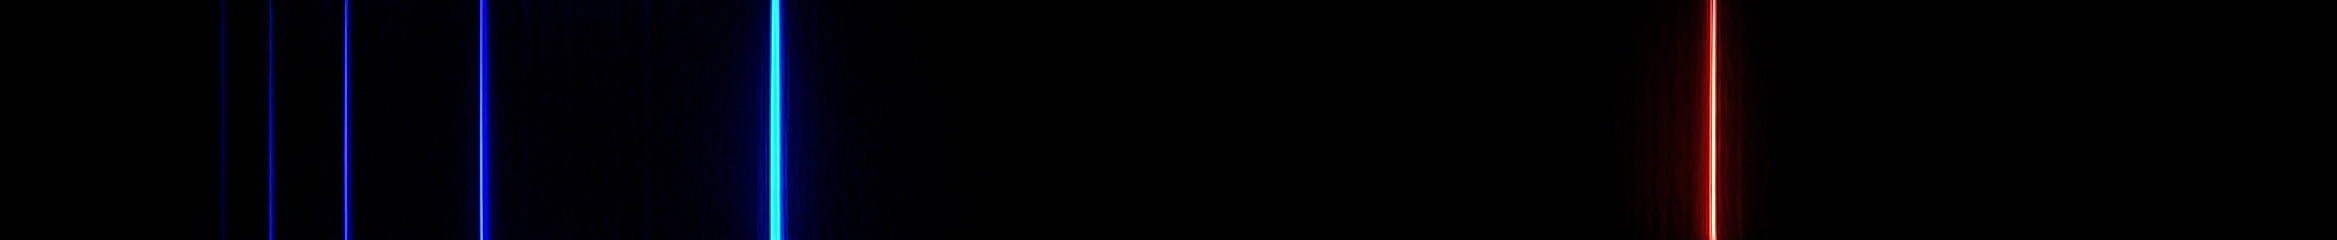
\includegraphics[width = .6\columnwidth]{atomuhr/wasserstoffSpektrum.jpg}
	\caption{Wasserstoffspektrum \cite{pic:wasserstoffspektrum}} 
	\label{atomuhr:wasserstoffspektrum}
\end{figure}

Auf der Abbildung \ref{atomuhr:wasserstoffspektrum} sieht man das
Frequenzspektrum der sogenannte Balmer-Serie des Wasserstoffs, welche
zuf"alligerweise im sichtbaren Bereich ist. Die rote Linie ganz rechts
ist die $H\alpha$-Linie. Die n"achste links $H\beta$ und so weiter.


\subsection{Feinstruktur"ubergang}
Damit jedoch ein solcher "Ubergang elektrisch verarbeitet werden kann,
muss es einen Effekt geben, bei welchem das Photon mit einer Frequenz
im Gigahertz Bereich ausgesendet wird.  Der Feinstruktur"ubergang ist
ein erster Schritt in diese Richtung.

Als das Wasserstoffspektrum genauer untersuchte wurde, bemerkte man,
dass die Spektrallinien nicht einfach sind. Wenn man beispielsweise die
$H\alpha$ Spektrallinie besser aufl"ost, so entdeckt man, dass diese
eine Linie aus zwei Linien besteht, welche sehr nahe beieinander
liegen (Abbildung \ref{atomuhr:fineStructure}).

\begin{figure}
	\centering
	
\includegraphics[width = .6\columnwidth]{atomuhr/fine_structure_hydrogen.png}
	\caption{$H\alpha$-Linie stark vergr"ossert, erkennbare
          Doppellinie \cite{pic:wasserstoff_feinstruktur}}
        \label{atomuhr:fineStructure}
\end{figure}

\begin{itemize}
	\item[]  $H = \textcolor{red}{H_0}+ \textcolor{blue}{W_{SB}} + 
		\textcolor{green}{W_M} + \textcolor{violet}{W_D} $
	\item[]  $H$: Hamiltonoperator mit Spin- und relativistischer Korrekturen
	\item[]  \textcolor{red}{$H_0$}: Hamiltonoperator ohne Spin
          aus Kapitel \ref{chapter:wasserstoff}
	\item[]  \textcolor{blue}{$W_{SB}$}: Spin Bahn Kopplung
	\item[]  \textcolor{green}{$W_M$}: Korrektur kin. Energie
	\item[]  \textcolor{violet}{$W_D$}: Korrektur pot. Energie
	
\end{itemize}
		
Auf die Korrekturfaktoren $W_M$ und $W_D$ wird hier nicht n"aher
eingegangen, da diese nur zu geringf"ugigen Korrekturen f"uhrt und
nicht f"ur die Doppellinie verantwortlich ist.

Der Hamiltonoperator ohne Spin beschreibt das Modell aus Kapitel
\ref{chapter:wasserstoff}.

Bei der Spin Bahn Kopplung geht es um die reine Betrachtung des
Elektrons.  Bei ihrer Bewegung um den Atomkern entsteht durch die
eigene Ladung ein magnetisches Feld.  Dieses Feld wechselwirkt nun mit
dem magnetischen Spin, den das Elektron auch noch besitzt.  Da das
Elektron entweder Spin \(+\frac{1}{2}\) oder \(-\frac{1}{2}\) hat,
entstehen geringf"ugig unterschiedliche Frequenzen bei einem
Quantensprung in das jeweilige Energielevel.

\begin{figure}
	\centering
	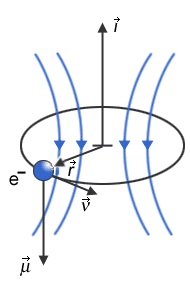
\includegraphics[width=.2\columnwidth]{atomuhr/feinstrukturelektron.jpg}
	\caption{Spin Bahn Kopplung \cite{pic:feinstruktur}}
	\label{atomuhr:spinbahn}
\end{figure}

\subsubsection{Notation Termsymbol}
Jedes Atom hat nun verschiedene Energiezust"ande, in denen sich
Elektronen befinden.  Dabei befinden sich die Elektronen in einem
bestimmten Sektor, welchem ein gewisser Bahndrehimpuls zugewiesen ist
(Abbildung \ref{atomuhr:bahndrehimpuls}).
\begin{figure}
	\centering
	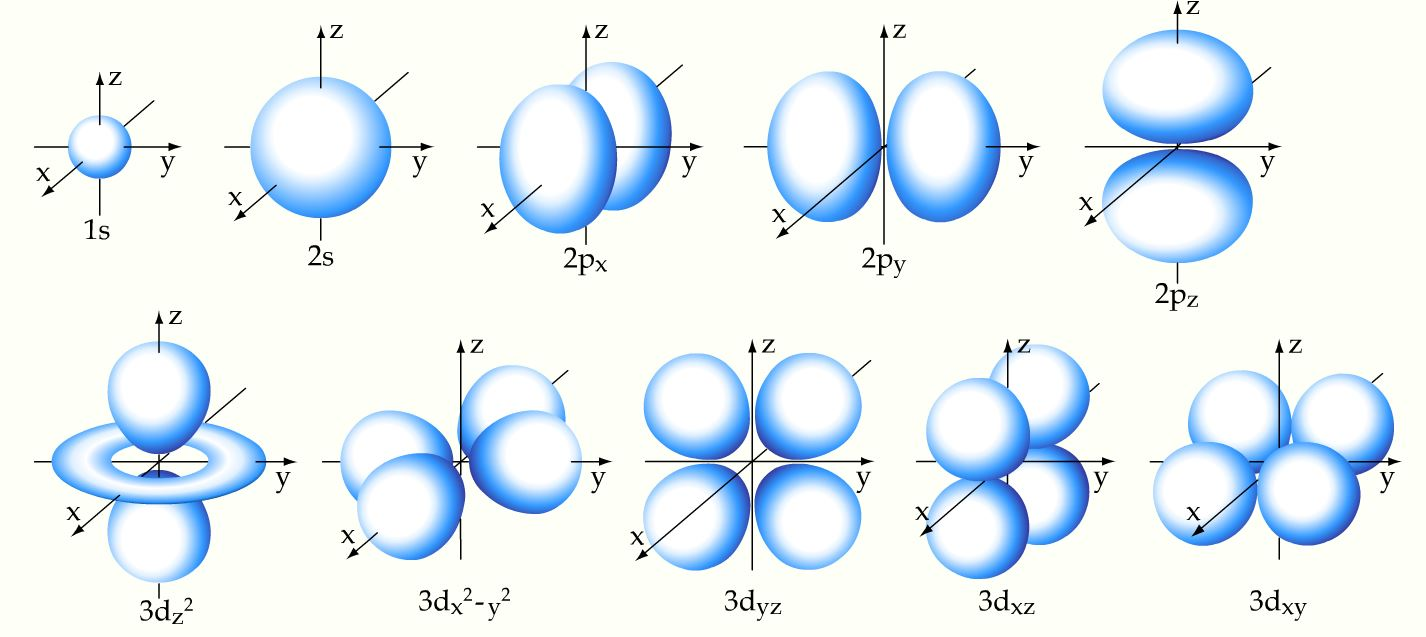
\includegraphics[width = 0.8\columnwidth]{atomuhr/orbitale.JPG}
	\caption{Wellenfunktionen zu verschiedenen Bahndrehimpulsen \cite{pic:orbitale}}
	\label{atomuhr:bahndrehimpuls}
\end{figure}
Ausserdem hat das Elektron zwei verschiedene Spinzust"ande in dem es
sich befinden kann.  Um den Zustand eines Elektrons zu beschreiben,
wurde die Termsymbol Notation entwickelt.  Diese wird nachfolgend kurz
erkl"art.

\begin{equation}
	\text{Termsymbol:} \quad ^NL _J
\end{equation}

wobei

\begin{equation}
	J = L + S
\end{equation}

$N:$ Entartungsgrad

$L:$ elektrische Bahndrehimpuls

$J:$ Gesamtdrehimpuls

$S:$ Spin Elektron

Dem elektrischen Bahndrehimpuls sind dabei den Zeichen die Zahlen in
Tabelle \ref{atomuhr:drehimpulsnotation} zugewiesen.

\begin{table}
	\centering	
	\begin{tabular}{llll}
		s & p & d & f \\
		1 & 2 & 3 & 4 \\
	\end{tabular}
	\caption{elektrische Bahndrehimpulse}
	\label{atomuhr:drehimpulsnotation}
\end{table}

Mit diesem Wissen l"asst sich nun ein Feinstruktur"ubergang ausrechnen. 
\begin{align*}
  &\text{"Ubergang \(^2P_{3/2} \rightarrow\,^2P_{1/2}\):} &\lambda &=
  \SI{2.76}{\centi\meter} &\nu &= \dfrac{c}{\lambda} =
  \SI{10.9}{\giga\hertz}
\end{align*}

Das ausgesendete Photon befindet sich bei diesen
Feinstruktur"uberg"angen in einem Bereich, in dem sie schon eher
genutzt werden k"onnte. F"ur Atomuhren wird jedoch der
Hyperfeinstruktur"ubergang genutzt.

\subsection{Hyperfeinstruktur"ubergang}
\label{sec:hyperf}
Der Feinstruktur"ubergang wurde entdeckt, als das Bohrsche Modell
experimentell genauer untersucht wurde. "Ahnlich ergeht es dem
Hyperfeinstruktur"ubergang. Als das Spektrum des Feinstruktur"ubergang
besser aufgel"ost werden konnte, ist aufgefallen, das es noch einen
weiteren Effekt gibt, welcher zu einer Aufspaltung eines Energielevels
beim Feinstruktur"ubergang f"uhrt. Dieser wurde
Hyperfeinstruktur"ubergang genannt und wird hier nun erkl"art.

Dieser Struktur"ubergang kann mithilfe der Wechselwirkung zwischen
Elektron und Kern erkl"art werden. Der Kern besitzt einen gewissen
Kernspin. Der magnetische Spin des Elektrons kann nun parallel oder
antiparallel zum Kern sein. Was zu unterschiedlichen Energieniveaus
f"uhrt.

Beim Wasserstoff, welches im Grundzustand besetzt ist, f"uhrt das zu
einer Wellenl"ange von $\lambda = \SI{21}{\centi\meter}$, was einer
Frequenz von $\nu = \SI{1.42}{\giga\hertz}$ entspricht. Das ist eine
Frequenz, welche sich sehr gut mit elektronischen Ger"aten verarbeiten
l"asst.

\subsection{Alkalimetalle}
Gleich wie Wasserstoff geh"ort auch Rubidium und C"asium zu den
Alkalimetallen. Speziell an dieser Gruppe von Elementen ist, dass sie
nur ein freies Elektron in der letzten besetzten Schale haben.

Da alle Atome Edelgaskonfiguration anstreben, wollen die Alkalimetalle
dieses freie Elektron m"oglichst abgeben und sind dadurch relativ
Reaktionsfreudig.  Die abgeschlossenen Schalen sind elektrisch gesehen
neutral.  Weshalb die Alkalimetalle mutmasslich f"ur Atomuhren
gebraucht werden.  Da das Frequenzspektrum bei einem Valenzelektron
einfacher zu verstehen ist, als bei anderen Atomgruppen mit mehreren
Valenzelektronen.

Rubidium hat einen Hyperfrequenz"ubergang von $\nu =
\SI{6.834}{\giga\hertz}$. Die h"ohere Frequenz im Vergleich zum
Wasserstoffatom l"asst sich damit erkl"aren, dass sich das
Valenzelektron weiter weg vom Kern befindet.  Die Kraft auf die
Wechselwirkung ist somit kleiner.

\section{Technische Betrachtung}
In der technischen Betrachtung in diesem Abschnitt wird die
Funktionsf"ahigkeit des Rubidium-Frequenznormals LPRO-101 aufgezeigt.
Das Datenblatt dieser Atomuhr kann unter \cite{datasheet:lpro}
gefunden werden.  Ein ausf"uhrliches Datenblatt ist unter
\cite{datasheet:prs10m} zu finden, in welchem ein anderes Modell
erkl"ahrt wird.  Die Funktionsbeschreibung ist jedoch besser.

Solche Rubidium Frequenznormale besitzen die Gr"osse einer Handfl"ache
und erreichen eine Genauigkeit von ungef"ahr \num{e-9}.  In der
Abbildung \ref{fig:techBlock} ist der schematische Aufbau einer
solchen Atomuhr aufgezeigt.  Die Hauptfunktion dieser Schaltung ist
ein Regelkreis, welcher sich auf den Hyperfeinstrucktur"ubergang des
Rubidium-87 ein regelt, welcher bei \SI{6.8346875}{\giga\hertz} liegt.

\begin{figure}
  \centering
  \begin{tikzpicture}
    [node distance=1.3cm]

    \tikzstyle{conn} = [->,shorten >=0.1cm,>=stealth',very thick];

    \tikzstyle{connLamp} = [->, decorate, 
                            decoration={snake,
                              amplitude=1.5mm,
                              segment length=1.7mm,
                              post length=2.7mm},
                            shorten >=0.1cm,
                            >=stealth', very thick,
                            color=red!50!black];

    \tikzstyle{connAbsorber} = [->, shorten >=0.1cm,
                                >=stealth', very thick];

    \tikzstyle{connHfgen} = [->, decorate,
                             decoration={snake,
                               amplitude=1.5mm,
                               segment length=9mm,
                               post length=2.5mm},
                             shorten >=0.1cm,
                             >=stealth',very thick];

    \tikzstyle{lamp} = [draw=red!50!black,
                        thick,circle,inner sep=1.5mm,
                        fill=red!30];

    \tikzstyle{absorber} = [draw, thin, circle,
                            shade, shading=radial,
                            inner color=blue!70];

    \tikzstyle{vcxo} = [draw, thick, rectangle, inner sep=5mm,
                        align=center, minimum width=2.7cm];
    \tikzstyle{hfgen} = [draw,thick, rectangle, inner sep=5mm];

    % drawing
    \node[lamp, minimum size=1.7cm] (lamp) {$^{87}$Ru};

    \node[absorber, minimum size=1.7cm] (absorber) [right=of lamp] {};

    \node (diode) [right=of absorber] {};

    \draw[semithick](diode) ++ (0.0,-1.0) to[empty photodiode]
                            ++ (0.0,2.0);

    \node[vcxo] (vcxo) [right=of diode] {\SI{20}{\mega\hertz}\\VCXO};

    \node[hfgen] (hfgen) [below=of absorber] {\(\times\)};

    \node[xshift=1cm] (note) [left=of hfgen] {\SI{6.8346875}{\giga\hertz}};

    % connections
    \draw[connLamp] (lamp.east) -- (absorber.west);
    \draw[connAbsorber, shorten >=0.4cm] (absorber.east) -- (diode.west);
    \draw[conn] (diode.east) ++ (0.3cm,0.0) -- (vcxo.west);
    \draw[conn] (vcxo.south) |- (hfgen.east);
    \draw[connHfgen] (hfgen.north) -- (absorber.south);
\end{tikzpicture}
  \caption{Schematischer Aufbau einer Rubidium Atomuhr}
  \label{fig:techBlock}
\end{figure}

\subsection{Funktionsweise}
Die Rubidium-87 Entladungslampe wird angeregt und emittiert Licht bei
ca. \SI{780}{\nano\meter}.  Dieses Licht wird in die Resonator-Kammer
geleitet, in welcher ein Absorptionsgas aus Rubidium-87 vorhanden ist.
Weiter ist in der Entladungslampe und der Resonatorkammer ein
Filtergas aus Rubidium-85 vorhanden.  In der Abbildung
\ref{fig:uebergaenge} ist die Filterung dargestellt.

\begin{figure}
  \centering
  \subfigure[ohne \SI{6.8}{\giga\hertz} Anregung]{
    \begin{tikzpicture}
  \tikzstyle{trans} = [->,>=stealth',very thick];
  \tikzstyle{photon} = [->, decorate, 
                        decoration={snake,
                          amplitude=1.5mm,
                          segment length=3mm,
                          post length=2mm},
 %                       shorten >=3mm,
                        >=stealth', very thick];


  \draw (0,0) node[above left] {5s} --++ (7.5cm,0)
  node[above right] {ohne \SI{6.8}{\giga\hertz}};
  \draw (0,0.4cm) --++ (7.5cm,0);
  \draw (0,4cm) node[left] {5p} --++ (7.5cm,0);

  % lamp
  \draw[very thick] (0,0cm)   --++ (1.5cm,0);
  \draw[very thick] (0,0.4cm) --++ (1.5cm,0);

  \draw[very thick] (0,4cm)   --++ (1.5cm,0);

  \draw[trans, red!70!black] (0.5cm,4cm) -- (0.5cm,0.4cm);
  \draw[trans, blue!70!black] (1cm,4cm) -- (1cm,0cm);

  \node[align=center] at (0.75cm,-1cm) {$^{87}$Rb\\Emission};

  % filter
  \draw[very thick] (3,0.4cm) --++ (1.5cm,0);
  \draw[very thick] (3,0.8cm) --++ (1.5cm,0);

  \draw[very thick] (3,4cm)   --++ (1.5cm,0);

  \draw[trans, red!70!black] (3.5cm,0.4cm) -- (3.5cm,4cm);
  \draw[trans, red!70!black] (4cm,4cm) -- (4cm,0.4cm);

  \node[align=center] at (3.75cm,-1cm) {$^{85}$Rb\\Filter};

  % resonator
  \draw[semithick] (6,0cm)   --++ (1.5cm,0);
  \draw[line width=0.15cm] (6,0.4cm) --++ (1.5cm,0);

  \draw[very thick] (6,4cm)   --++ (1.5cm,0);

  \draw[trans, red!70!black] (6.5cm,4cm) -- (6.5cm,0.4cm);
  \draw[trans, blue!70!black] (7cm,0cm) -- (7cm,4cm);

  \node[align=center] at (6.75cm,-1cm) {$^{87}$Rb\\Resonator};

  % photons
  %   lamp
  \draw[photon, red!70!black] (1.3, 3cm) --++ (1.9cm,0);
  \draw[photon, blue!70!black] (1.5, 2cm) --++ (4.7cm,0);
\end{tikzpicture}}\\
  \subfigure[mit \SI{6.8}{\giga\hertz} Anregung]{
    \begin{tikzpicture}
  \tikzstyle{trans} = [->,>=stealth',very thick];
  \tikzstyle{photon} = [->, decorate, 
                        decoration={snake,
                          amplitude=1.5mm,
                          segment length=3mm,
                          post length=2mm},
 %                       shorten >=3mm,
                        >=stealth', very thick];
  \tikzstyle{photonHFG} = [->, decorate,
                           decoration={snake,
                             amplitude=1.5mm,
                             segment length=9mm,
                             post length=2mm},
%                           shorten >=0.1cm,
                           >=stealth',very thick];


  \draw (0,0) node[above left] {5s} --++ (7.5cm,0)
  node[above right] {mit \SI{6.8}{\giga\hertz}};
  \draw (0,0.4cm) --++ (7.5cm,0);
  \draw (0,4cm) node[left] {5p} --++ (7.5cm,0);

  % lamp
  \draw[very thick] (0,0cm)   --++ (1.5cm,0);
  \draw[very thick] (0,0.4cm) --++ (1.5cm,0);

  \draw[very thick] (0,4cm)   --++ (1.5cm,0);

  \draw[trans, red!70!black] (0.5cm,4cm) -- (0.5cm,0.4cm);
  \draw[trans, blue!70!black] (1cm,4cm) -- (1cm,0cm);

  \node[align=center] at (0.75cm,-1cm) {$^{87}$Rb\\Emission};

  % filter
  \draw[very thick] (3,0.4cm) --++ (1.5cm,0);
  \draw[very thick] (3,0.8cm) --++ (1.5cm,0);

  \draw[very thick] (3,4cm)   --++ (1.5cm,0);

  \draw[trans, red!70!black] (3.5cm,0.4cm) -- (3.5cm,4cm);
  \draw[trans, red!70!black] (4cm,4cm) -- (4cm,0.4cm);

  \node[align=center] at (3.75cm,-1cm) {$^{85}$Rb\\Filter};

  % resonator
  \draw[very thick] (6,0cm)   --++ (1.5cm,0);
  \draw[very thick] (6,0.4cm) --++ (1.5cm,0);

  \draw[very thick] (6,4cm)   --++ (1.5cm,0);

  \draw[trans, red!70!black] (6.5cm,4cm) -- (6.5cm,0.4cm);
  \draw[trans, orange!70!black] (6.5cm,0.4cm) -- (6.5cm,0cm);
  \draw[trans, blue!70!black] (7cm,0cm) -- (7cm,4cm);

  \node[align=center] at (6.75cm,-1cm) {$^{87}$Rb\\Resonator};

  % photons
  %   lamp
  \draw[photon, red!70!black] (1.3, 3cm) --++ (1.9cm,0);
  \draw[photon, blue!70!black] (1.5, 2cm) --++ (4.7cm,0);
  %   hf
  \draw[photonHFG, orange!70!black] (9cm, 3cm) --++ (-1.7cm,0);
\end{tikzpicture}}
  \caption{Energie"uberh"ange in einer Rubidium Atomuhr}
  \label{fig:uebergaenge}
\end{figure}


Die Entladungslampe emittiert zwei sehr "ahnliche Frequenzen, da das
untere Energieniveau 5s der Rubidium-87 Atome nur durch ihren
unterschiedlichen Spin aufgeteilt wird.  Die zur Filterung
eingesetzten Rubidium-85 Atome besitzen ein leicht verschobenes
unteres Energieniveau, welches mit einem der beiden 5s Energieniveaus
von Rubidium-87 "ubereinstimmt.  Diese "Ubereinstimmung ist f"ur die
Funktionsweise der Rubidium Atomuhr von grosser Bedeutung, da man
damit eine der beiden Emittierten Frequenzen des Rubidium-87
herausfiltern kann.  So erreicht nur eine der beiden Frequenzen die
Resonator-Kammer.

Im Resonator absorbiert das Rubidium-87 die eintreffenden
Photonen. Das Elektron steigt in das h"ohere Energieniveau 5p auf und
f"allt spontan mit einer Wahrscheinlichkeit von \SI{50}{\percent} in
eine der beiden unteren Energieniveaus von 5s zur"uck.  Mit der Zeit
sammeln sich mehr Elektronen im oberen der beiden Energieniveaus von
5s an, da keine Photonen mit dieser ben"otigten Frequenz zum Resonator
(Filterung durch Rubidium-85) gelangen.  Es werden weniger Photonen
absorbiert, was der Detektor messen kann.  (Eine weitere Anwendung,
welche mit den Energie"uberg"angen arbeitet ist der Laser, zu finden
im Kapitel \ref{chapter:laser}.)

Der Detektor steuert einen spannungsgesteuerten Oszillator (VCXO) an,
welcher eine Frequenz um \SI{20}{\mega\hertz} ausgibt.  Dieses Signal
wird mit einem Multiplizierer auf die Frequenz des
Hyperfeinstruktur"ubergang hinauf multipliziert.

Diese hinauf multiplizierte Frequenz liegt nun im Mikrowellenbereich
und wird zur"uck in den Resonator geleitet.  Wird nun die Frequenz von
\SI{6.8346875}{\giga\hertz} genau getroffen, wird am VCXO genau
\SI{20}{\mega\hertz} ausgegeben.  Weiter entspricht die
Mikrowellenstrahlung nun genau dem Hyperfeinstrucktur"ubergang, was zu
einer stimulierten Emission f"uhrt.  Durch diese stimulierte Emission
wird die Entv"olkerung des untersten Energiezustand von 5s aufgehoben.
Es stehen nun wieder Elektronen zur Verf"uhgung, welche Photonen
absorbieren k"onnen, was zu einer Abdunklung des Detektors f"uhrt.

Der ganze Regelkreis regelt somit auf die maximale Absorption im
Resonator und f"uhrt zu einer sehr genauen Ausgangsfrquenz von
\SI{20}{\mega\hertz}.

\subsection{Tuning}
Es stellt sich nun die Frage, wie ein solcher Regelkreis abgeglichen
werden kann.  Zum Beispiel m"ussen die GNSS Satelliten untereinander
und mit der Bodenstation synchronisiert werden.  Wie man in den
quantenmechanischen Betrachtungen gesehen hat, h"angt der
Hyperfeinstruktur"ubergang (\ref{sec:hyperf}) nur vom Magnetfeld des
Atomkerns und des Spin Magnetfelds ab.

Nun kann man diese Magnetfelder mit einem externen Magnetfeld st"oren,
was zu einer Frequenzverschiebung des Hyperfeinstrucktur"ubergangs
f"uhrt.  Das Magnetfeld wird wie in Abbildung \ref{fig:tuning}
dargestellt, am Resonator angelegt.  Mit dieser St"orung kann nun die
gew"unschte Frequenz mit einer genaueren Caesium Atomuhr oder dem GPS
Takt abgeglichen werden.

Wie stark sich nun diese Frequenz durch eine magnetische St"orung
beeinflussen l"asst, wird im n"achsten Abschnitt ausgerechnet.

\begin{figure}
  \centering
  \begin{tikzpicture}
    [node distance=1.3cm]

    \tikzstyle{conn} = [->,shorten >=0.1cm,>=stealth',very thick];

    \tikzstyle{connLamp} = [->, decorate, 
                            decoration={snake,
                              amplitude=1.5mm,
                              segment length=1.7mm,
                              post length=2.7mm},
                            shorten >=0.1cm,
                            >=stealth', very thick,
                            color=red!50!black];

    \tikzstyle{connAbsorber} = [->, shorten >=0.1cm,
                                >=stealth', very thick];

    \tikzstyle{connHfgen} = [->, decorate,
                             decoration={snake,
                               amplitude=1.5mm,
                               segment length=9mm,
                               post length=2.5mm},
                             shorten >=0.1cm,
                             >=stealth',very thick];

    \tikzstyle{lamp} = [draw=red!50!black,
                        thick,circle,inner sep=1.5mm,
                        fill=red!30];

    \tikzstyle{absorber} = [draw, thin, circle,
                            shade, shading=radial,
                            inner color=blue!70];

    \tikzstyle{vcxo} = [draw, thick, rectangle, inner sep=5mm,
                        align=center, minimum width=2.7cm];
    \tikzstyle{hfgen} = [draw,thick, rectangle, inner sep=5mm];

    % drawing
    \node[lamp, minimum size=1.7cm] (lamp) {$^{87}$Ru};

    \node[absorber, minimum size=1.7cm] (absorber) [right=of lamp] {};

    \node (diode) [right=of absorber] {};

    \draw[semithick](diode) ++ (0.0,-1.0) to[empty photodiode]
                            ++ (0.0,2.0);

    \node[vcxo] (vcxo) [right=of diode]
                       {\SI{\approx20}{\mega\hertz}\\VCXO};

    \node[hfgen] (hfgen) [below=of absorber] {\(\times\)};

    \node[xshift=1cm] (note) [left=of hfgen]
                                  {\SI{\approx6.8346875}{\giga\hertz}};

    % connections
    \draw[connLamp] (lamp.east) -- (absorber.west);
    \draw[connAbsorber, shorten >=0.4cm] (absorber.east) -- (diode.west);
    \draw[conn] (diode.east) ++ (0.3cm,0.0) -- (vcxo.west);
    \draw[conn] (vcxo.south) |- (hfgen.east);
    \draw[connHfgen] (hfgen.north) -- (absorber.south);

    % B field
    \foreach \x in {-1.25, -0.75, -0.25, 0.25, 0.75, 1.25}
      \draw[->, >=stealth', very thick, green!50!black] (absorber) ++
      (\x,1.5cm) --++ (0.0,-3cm);
  \end{tikzpicture}
  \caption{Frequenztuning durch Magnetfeld-St"orung am Resonator
    (gr"un angelegtes Magnetfeld).}
  \label{fig:tuning}
\end{figure}

\subsection{Rechnung}

\subsubsection{Kern Magnetfeld}
Im Kapitel \ref{chapter:spin} wird der Spin im Magnetfeld beschrieben.
Will man nun das Kernmagnetfeld eines Rubidium Atoms bestimmen, so
ben"otigt man die Hyperfeinstrukturfrequenz.  Beim Rubidium Atom ist
dies \SI{6.8346875}{\giga\hertz}.  Formt man nun die gegebenen Formeln
um,

\begin{equation*}
  \Delta E = h\cdot\nu = \dfrac{\hbar e}{m_e}B_z
\end{equation*}
erh"alt man das f"ur das Elektron sp"urbar, gemittelte Kernmagnetfeld
eines Rubidiumatoms:

\begin{equation*}
  B_z = \dfrac{m_e\cdot2\pi\cdot\nu}{e} = \SI{244.2}{\milli\tesla}
\end{equation*}

Zum Vergleich, das Erdmagnetfeld variiert je nach Ort zwischen
\SIrange[range-phrase={ bis }, range-units=single]{30}{60}{\micro\tesla}.

\subsubsection{Enfluss des Erdmagnetfelds}
Wenn man nach dem Datenblatt \cite{datasheet:prs10m} eine magnetische
Abh"angigkeit von

\begin{equation*}
  \dfrac{\Delta f}{f} < 2\cdot 10^{-10} \text{ pro } \SI{100}{\micro\tesla}
\end{equation*}
annimmt, ergibt sich daraus eine Frequenz"anderung von \(\Delta
f=\SI{0.698}{\hertz}\).  Bei der Hyperfeinstrukturfrequenz von \(f =
\SI{6.8346875}{\giga\hertz}\) nur ein kleiner Beitrag.  Nach dem
Datenblatt l"asst sich die Ausgangsfrequenz um \SI{14}{\hertz}
ver"andern.  Somit kann der Einfluss des Erdmagnetfeld ohne Problem
"ubersteuert werden.

\section{Geschichte der Atomuhr}
\label{sec:gesch-der-atom}
Bereits 1879 hatte Lord Kelvin die Idee, Atome als Zeit und L"angen
Standard zu verwenden.  Erst 1949 wurde dann in der USA am National
Institute of Standards and Technology (NIST) die erste Atomuhr gebaut
\cite{ieee:nist}.  Diese Atomuhr verwendete Ammoniak bei einer
Frequenz von \SI{23.87}{\giga\hertz}.  Die Genauigkeit dieses Atomuhr
lag bei ca. 1 zu \num{e-7}.

Diese Genauigkeit ist noch nicht sehr eindr"ucklich, wenn man
vergleicht, dass ein normaler Quarzoszillator bei einer Genauigkeit
von ca. \num{e-5} und eine beheizter Quarzoszillator (OCXO) durch den
reduzierten Temperaturdrift im Bereich von \num{2e-8} liegt.

Mit der Ammoniak Atomuhr konnte aber das Prinzip der Atomuhr
aufgezeigt werden.  Welche 1952 mit der ersten Caesium Atomuhr NBS-1
weitergef"uhrt werden konnte.  Die Genauigkeit und Stabilit"at der
Caesium Atomuhren konnte soweit gesteigert werden, dass 1967 die
SI-Sekunde als Hyperfeinstruktur"ubergang von Caesium-133 definiert
wurde.  Das f"uhrt dazu, dass eine Sekunde mit \num{9192631770} Takten
aufgel"ost wird.  Somit ist die Genauigkeit auf
\SI{108.78}{\pico\second} beschr"ankt.

Andere Atomuhren, welche in der Zwischenzeit entwickelt wurden,
verwenden die Elemente Rubidium und Wasserstoff.  Beide verwenden
ebenfalls den Hyperfeinstruktur"ubergang.  Die Rubidium Atomuhren
k"onnen sehr einfach und g"unstig aufgebaut werden, besitzen jedoch
nicht die Genauigkeit von Caesium Atomuhren.  Genauer k"onnen die
Wasserstoffatomuhren gebaut werden, ben"otigen jedoch eine komplexere
K"uhlung der Atome.

Will man eine genauere Aufl"osung erreichen, gen"ugt es nicht die
Hyperfeinstruktur"uberg"ange zu benutzen.  Man muss eine h"ohere
Taktung erreichen.  Diese h"oheren Taktungen k"onnen erreicht werden,
wenn Atome mit Spektrallinien im optischen Bereich verwendet werden.
Lange konnte dieser Bereich nicht genutzt werden, da diese hohen
Takte mit elektronischen Regelkreisen nicht gemessen werden konnten.

Gl"ucklicherweise wurde 1998 der Frequenzkamm entdeckt
\cite{SdW:kamm}.  Mit dessen Hilfe k"onnen Frequenzen im optischen
Spektrum mit einer Schwebung in den technisch messbaren
Frequenzbereich gebracht werden.  Diese Technologie erm"oglichte es
andere Atome zu verwenden, mit welchen man 2014 eine Genauigkeit von
\num{e-18} erreichte, was ca. einer Sekunde auf das Alter des
Universums entspricht.  In der Abbildung \ref{fig:periode} ist eine
nicht abschiessende Auflistung der verwendeten Elemente in Atomuhren
dargestellt.

\begin{figure}
  \centering
  \newcommand{\CommonElementTextFormat}[4]
{
  \begin{minipage}{2.2cm}
    \centering {\textbf{#1} \hfill #2}%
    \linebreak \linebreak {\textbf{#3}}%
    \linebreak \linebreak {{#4}}
  \end{minipage}
}

\newcommand{\NaturalElementTextFormat}[4]
{
  \CommonElementTextFormat{#1}{#2}{\Huge {#3}}{#4}
}

\newcommand{\SyntheticElementTextFormat}[4]
{
  \CommonElementTextFormat{#1}{#2}{\Huge #3}{#4}
}


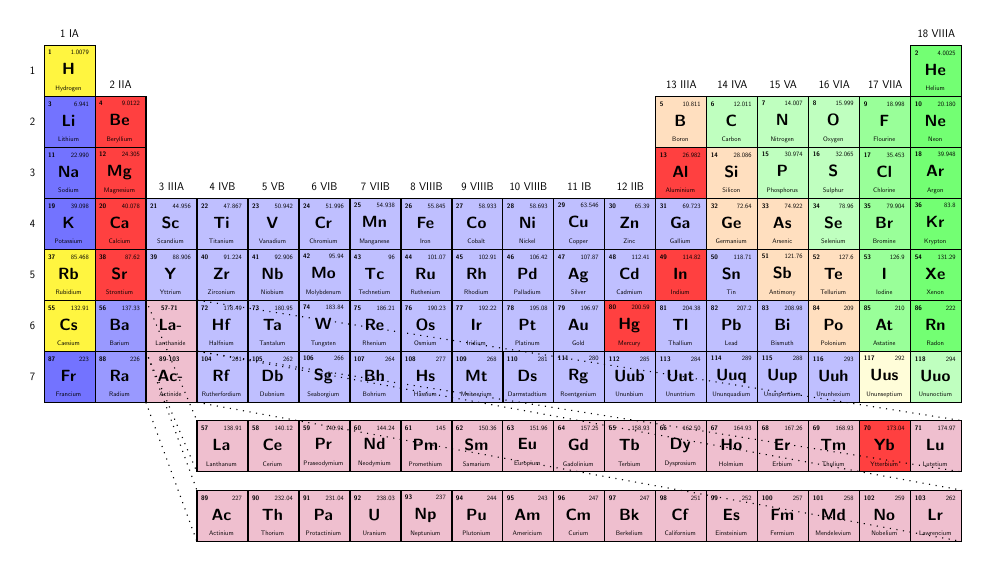
\begin{tikzpicture}[font=\sffamily, scale=\textwidth/51.5cm, transform shape]
  
  %% Fill Color Styles
  \tikzstyle{ElementFill} = [fill=yellow!15]
  \tikzstyle{AlkaliMetalFill} = [fill=blue!55]
  \tikzstyle{AlkalineEarthMetalFill} = [fill=blue!40]
  \tikzstyle{MetalFill} = [fill=blue!25]
  \tikzstyle{MetalloidFill} = [fill=orange!25]
  \tikzstyle{NonmetalFill} = [fill=green!25]
  \tikzstyle{HalogenFill} = [fill=green!40]
  \tikzstyle{NobleGasFill} = [fill=green!55]
  \tikzstyle{LanthanideActinideFill} = [fill=purple!25]
  \tikzstyle{AtomicClockElecFill} = [fill=yellow!75]
  \tikzstyle{AtomicClockOpticFill} = [fill=red!75]
  
  %% Element Styles
  \tikzstyle{Element} = [draw=black, ElementFill,
  minimum width=2.75cm, minimum height=2.75cm, node distance=2.75cm]
  \tikzstyle{AlkaliMetal} = [Element, AlkaliMetalFill]
  \tikzstyle{AlkalineEarthMetal} = [Element, AlkalineEarthMetalFill]
  \tikzstyle{Metal} = [Element, MetalFill]
  \tikzstyle{Metalloid} = [Element, MetalloidFill]
  \tikzstyle{Nonmetal} = [Element, NonmetalFill]
  \tikzstyle{Halogen} = [Element, HalogenFill]
  \tikzstyle{NobleGas} = [Element, NobleGasFill]
  \tikzstyle{LanthanideActinide} = [Element, LanthanideActinideFill]
  \tikzstyle{AtomicClockElec} = [Element, AtomicClockElecFill]
  \tikzstyle{AtomicClockOptic} = [Element, AtomicClockOpticFill]
  \tikzstyle{PeriodLabel} = [font={\sffamily\LARGE}, node distance=2.0cm]
  \tikzstyle{GroupLabel} = [font={\sffamily\LARGE}, minimum width=2.75cm, node distance=2.0cm]
  \tikzstyle{TitleLabel} = [font={\sffamily\Huge\bfseries}]
  
  %% Group 1 - IA
  \node[name=H, AtomicClockElec] {\NaturalElementTextFormat{1}{1.0079}{H}{Hydrogen}};
  \node[name=Li, below of=H, AlkaliMetal] {\NaturalElementTextFormat{3}{6.941}{Li}{Lithium}};
  \node[name=Na, below of=Li, AlkaliMetal] {\NaturalElementTextFormat{11}{22.990}{Na}{Sodium}};
  \node[name=K, below of=Na, AlkaliMetal] {\NaturalElementTextFormat{19}{39.098}{K}{Potassium}};
  \node[name=Rb, below of=K, AtomicClockElec] {\NaturalElementTextFormat{37}{85.468}{Rb}{Rubidium}};
  \node[name=Cs, below of=Rb, AtomicClockElec] {\NaturalElementTextFormat{55}{132.91}{Cs}{Caesium}};
  \node[name=Fr, below of=Cs, AlkaliMetal] {\NaturalElementTextFormat{87}{223}{Fr}{Francium}};
  
  %% Group 2 - IIA
  \node[name=Be, right of=Li, AtomicClockOptic] {\NaturalElementTextFormat{4}{9.0122}{Be}{Beryllium}};
  \node[name=Mg, below of=Be, AtomicClockOptic] {\NaturalElementTextFormat{12}{24.305}{Mg}{Magnesium}};
  \node[name=Ca, below of=Mg, AtomicClockOptic] {\NaturalElementTextFormat{20}{40.078}{Ca}{Calcium}};
  \node[name=Sr, below of=Ca, AtomicClockOptic] {\NaturalElementTextFormat{38}{87.62}{Sr}{Strontium}};
  \node[name=Ba, below of=Sr, AlkalineEarthMetal] {\NaturalElementTextFormat{56}{137.33}{Ba}{Barium}};
  \node[name=Ra, below of=Ba, AlkalineEarthMetal] {\NaturalElementTextFormat{88}{226}{Ra}{Radium}};
  
  %% Group 3 - IIIB
  \node[name=Sc, right of=Ca, Metal] {\NaturalElementTextFormat{21}{44.956}{Sc}{Scandium}};
  \node[name=Y, below of=Sc, Metal] {\NaturalElementTextFormat{39}{88.906}{Y}{Yttrium}};
  \node[name=LaLu, below of=Y, LanthanideActinide] {\NaturalElementTextFormat{57-71}{}{La-}{Lanthanide}};
  \node[name=AcLr, below of=LaLu, LanthanideActinide] {\NaturalElementTextFormat{89-103}{}{Ac-}{Actinide}};
  % \node[name=LaLu, below of=Y, LanthanideActinide] {\NaturalElementTextFormat{57-71}{}{La-Lu}{Lanthanide}};
  % \node[name=AcLr, below of=LaLu, LanthanideActinide] {\NaturalElementTextFormat{89-103}{}{Ac-Lr}{Actinide}};
  
  %% Group 4 - IVB
  \node[name=Ti, right of=Sc, Metal] {\NaturalElementTextFormat{22}{47.867}{Ti}{Titanium}};
  \node[name=Zr, below of=Ti, Metal] {\NaturalElementTextFormat{40}{91.224}{Zr}{Zirconium}};
  \node[name=Hf, below of=Zr, Metal] {\NaturalElementTextFormat{72}{178.49}{Hf}{Halfnium}};
  \node[name=Rf, below of=Hf, Metal] {\SyntheticElementTextFormat{104}{261}{Rf}{Rutherfordium}};
  
  %% Group 5 - VB
  \node[name=V, right of=Ti, Metal] {\NaturalElementTextFormat{23}{50.942}{V}{Vanadium}};
  \node[name=Nb, below of=V, Metal] {\NaturalElementTextFormat{41}{92.906}{Nb}{Niobium}};
  \node[name=Ta, below of=Nb, Metal] {\NaturalElementTextFormat{73}{180.95}{Ta}{Tantalum}};
  \node[name=Db, below of=Ta, Metal] {\SyntheticElementTextFormat{105}{262}{Db}{Dubnium}};
  
  %% Group 6 - VIB
  \node[name=Cr, right of=V, Metal] {\NaturalElementTextFormat{24}{51.996}{Cr}{Chromium}};
  \node[name=Mo, below of=Cr, Metal] {\NaturalElementTextFormat{42}{95.94}{Mo}{Molybdenum}};
  \node[name=W, below of=Mo, Metal] {\NaturalElementTextFormat{74}{183.84}{W}{Tungsten}};
  \node[name=Sg, below of=W, Metal] {\SyntheticElementTextFormat{106}{266}{Sg}{Seaborgium}};
  
  %% Group 7 - VIIB
  \node[name=Mn, right of=Cr, Metal] {\NaturalElementTextFormat{25}{54.938}{Mn}{Manganese}};
  \node[name=Tc, below of=Mn, Metal] {\NaturalElementTextFormat{43}{96}{Tc}{Technetium}};
  \node[name=Re, below of=Tc, Metal] {\NaturalElementTextFormat{75}{186.21}{Re}{Rhenium}};
  \node[name=Bh, below of=Re, Metal] {\SyntheticElementTextFormat{107}{264}{Bh}{Bohrium}};
  
  %% Group 8 - VIIIB
  \node[name=Fe, right of=Mn, Metal] {\NaturalElementTextFormat{26}{55.845}{Fe}{Iron}};
  \node[name=Ru, below of=Fe, Metal] {\NaturalElementTextFormat{44}{101.07}{Ru}{Ruthenium}};
  \node[name=Os, below of=Ru, Metal] {\NaturalElementTextFormat{76}{190.23}{Os}{Osmium}};
  \node[name=Hs, below of=Os, Metal] {\SyntheticElementTextFormat{108}{277}{Hs}{Hassium}};
  
  %% Group 9 - VIIIB
  \node[name=Co, right of=Fe, Metal] {\NaturalElementTextFormat{27}{58.933}{Co}{Cobalt}};
  \node[name=Rh, below of=Co, Metal] {\NaturalElementTextFormat{45}{102.91}{Rh}{Rhodium}};
  \node[name=Ir, below of=Rh, Metal] {\NaturalElementTextFormat{77}{192.22}{Ir}{Iridium}};
  \node[name=Mt, below of=Ir, Metal] {\SyntheticElementTextFormat{109}{268}{Mt}{Meitnerium}};
  
  %% Group 10 - VIIIB
  \node[name=Ni, right of=Co, Metal] {\NaturalElementTextFormat{28}{58.693}{Ni}{Nickel}};
  \node[name=Pd, below of=Ni, Metal] {\NaturalElementTextFormat{46}{106.42}{Pd}{Palladium}};
  \node[name=Pt, below of=Pd, Metal] {\NaturalElementTextFormat{78}{195.08}{Pt}{Platinum}};
  \node[name=Ds, below of=Pt, Metal] {\SyntheticElementTextFormat{110}{281}{Ds}{Darmstadtium}};
  
  %% Group 11 - IB
  \node[name=Cu, right of=Ni, Metal] {\NaturalElementTextFormat{29}{63.546}{Cu}{Copper}};
  \node[name=Ag, below of=Cu, Metal] {\NaturalElementTextFormat{47}{107.87}{Ag}{Silver}};
  \node[name=Au, below of=Ag, Metal] {\NaturalElementTextFormat{79}{196.97}{Au}{Gold}};
  \node[name=Rg, below of=Au, Metal] {\SyntheticElementTextFormat{111}{280}{Rg}{Roentgenium}};
  
  %% Group 12 - IIB
  \node[name=Zn, right of=Cu, Metal] {\NaturalElementTextFormat{30}{65.39}{Zn}{Zinc}};
  \node[name=Cd, below of=Zn, Metal] {\NaturalElementTextFormat{48}{112.41}{Cd}{Cadmium}};
  \node[name=Hg, below of=Cd, AtomicClockOptic] {\NaturalElementTextFormat{80}{200.59}{Hg}{Mercury}};
  \node[name=Uub, below of=Hg, Metal] {\SyntheticElementTextFormat{112}{285}{Uub}{Ununbium}};
  
  %% Group 13 - IIIA
  \node[name=Ga, right of=Zn, Metal] {\NaturalElementTextFormat{31}{69.723}{Ga}{Gallium}};
  \node[name=Al, above of=Ga, AtomicClockOptic] {\NaturalElementTextFormat{13}{26.982}{Al}{Aluminium}};
  \node[name=B, above of=Al, Metalloid] {\NaturalElementTextFormat{5}{10.811}{B}{Boron}};
  \node[name=In, below of=Ga, AtomicClockOptic] {\NaturalElementTextFormat{49}{114.82}{In}{Indium}};
  \node[name=Tl, below of=In, Metal] {\NaturalElementTextFormat{81}{204.38}{Tl}{Thallium}};
  \node[name=Uut, below of=Tl, Metal] {\SyntheticElementTextFormat{113}{284}{Uut}{Ununtrium}};
  
  %% Group 14 - IVA
  \node[name=C, right of=B, Nonmetal] {\NaturalElementTextFormat{6}{12.011}{C}{Carbon}};
  \node[name=Si, below of=C, Metalloid] {\NaturalElementTextFormat{14}{28.086}{Si}{Silicon}};
  \node[name=Ge, below of=Si, Metalloid] {\NaturalElementTextFormat{32}{72.64}{Ge}{Germanium}};
  \node[name=Sn, below of=Ge, Metal] {\NaturalElementTextFormat{50}{118.71}{Sn}{Tin}};
  \node[name=Pb, below of=Sn, Metal] {\NaturalElementTextFormat{82}{207.2}{Pb}{Lead}};
  \node[name=Uuq, below of=Pb, Metal] {\SyntheticElementTextFormat{114}{289}{Uuq}{Ununquadium}};
  
  %% Group 15 - VA
  \node[name=N, right of=C, Nonmetal] {\NaturalElementTextFormat{7}{14.007}{N}{Nitrogen}};
  \node[name=P, below of=N, Nonmetal] {\NaturalElementTextFormat{15}{30.974}{P}{Phosphorus}};
  \node[name=As, below of=P, Metalloid] {\NaturalElementTextFormat{33}{74.922}{As}{Arsenic}};
  \node[name=Sb, below of=As, Metalloid] {\NaturalElementTextFormat{51}{121.76}{Sb}{Antimony}};
  \node[name=Bi, below of=Sb, Metal] {\NaturalElementTextFormat{83}{208.98}{Bi}{Bismuth}};
  \node[name=Uup, below of=Bi, Metal] {\SyntheticElementTextFormat{115}{288}{Uup}{Ununpentium}};
  
  %% Group 16 - VIA
  \node[name=O, right of=N, Nonmetal] {\NaturalElementTextFormat{8}{15.999}{O}{Oxygen}};
  \node[name=S, below of=O, Nonmetal] {\NaturalElementTextFormat{16}{32.065}{S}{Sulphur}};
  \node[name=Se, below of=S, Nonmetal] {\NaturalElementTextFormat{34}{78.96}{Se}{Selenium}};
  \node[name=Te, below of=Se, Metalloid] {\NaturalElementTextFormat{52}{127.6}{Te}{Tellurium}};
  \node[name=Po, below of=Te, Metalloid] {\NaturalElementTextFormat{84}{209}{Po}{Polonium}};
  \node[name=Uuh, below of=Po, Metal] {\SyntheticElementTextFormat{116}{293}{Uuh}{Ununhexium}};
  
  %% Group 17 - VIIA
  \node[name=F, right of=O, Halogen] {\NaturalElementTextFormat{9}{18.998}{F}{Flourine}};
  \node[name=Cl, below of=F, Halogen] {\NaturalElementTextFormat{17}{35.453}{Cl}{Chlorine}};
  \node[name=Br, below of=Cl, Halogen] {\NaturalElementTextFormat{35}{79.904}{Br}{Bromine}};
  \node[name=I, below of=Br, Halogen] {\NaturalElementTextFormat{53}{126.9}{I}{Iodine}};
  \node[name=At, below of=I, Halogen] {\NaturalElementTextFormat{85}{210}{At}{Astatine}};
  \node[name=Uus, below of=At, Element] {\SyntheticElementTextFormat{117}{292}{Uus}{Ununseptium}}; 
  
  %% Group 18 - VIIIA
  \node[name=Ne, right of=F, NobleGas] {\NaturalElementTextFormat{10}{20.180}{Ne}{Neon}};
  \node[name=He, above of=Ne, NobleGas] {\NaturalElementTextFormat{2}{4.0025}{He}{Helium}};
  \node[name=Ar, below of=Ne, NobleGas] {\NaturalElementTextFormat{18}{39.948}{Ar}{Argon}};
  \node[name=Kr, below of=Ar, NobleGas] {\NaturalElementTextFormat{36}{83.8}{Kr}{Krypton}};
  \node[name=Xe, below of=Kr, NobleGas] {\NaturalElementTextFormat{54}{131.29}{Xe}{Xenon}};
  \node[name=Rn, below of=Xe, NobleGas] {\NaturalElementTextFormat{86}{222}{Rn}{Radon}};
  \node[name=Uuo, below of=Rn, Nonmetal] {\SyntheticElementTextFormat{118}{294}{Uuo}{Ununoctium}}; 
  
  %% Period
  \node[name=Period1, left of=H, PeriodLabel] {1};
  \node[name=Period2, left of=Li, PeriodLabel] {2};
  \node[name=Period3, left of=Na, PeriodLabel] {3}; 
  \node[name=Period4, left of=K, PeriodLabel] {4}; 
  \node[name=Period5, left of=Rb, PeriodLabel] {5};
  \node[name=Period6, left of=Cs, PeriodLabel] {6};
  \node[name=Period7, left of=Fr, PeriodLabel] {7};
  
  %% Group
  \node[name=Group1, above of=H, GroupLabel] {1 \hfill IA};
  \node[name=Group2, above of=Be, GroupLabel] {2 \hfill IIA};
  \node[name=Group3, above of=Sc, GroupLabel] {3 \hfill IIIA};
  \node[name=Group4, above of=Ti, GroupLabel] {4 \hfill IVB};
  \node[name=Group5, above of=V, GroupLabel] {5 \hfill VB};
  \node[name=Group6, above of=Cr, GroupLabel] {6 \hfill VIB};
  \node[name=Group7, above of=Mn, GroupLabel] {7 \hfill VIIB};
  \node[name=Group8, above of=Fe, GroupLabel] {8 \hfill VIIIB};
  \node[name=Group9, above of=Co, GroupLabel] {9 \hfill VIIIB};
  \node[name=Group10, above of=Ni, GroupLabel] {10 \hfill VIIIB};
  \node[name=Group11, above of=Cu, GroupLabel] {11 \hfill IB};
  \node[name=Group12, above of=Zn, GroupLabel] {12 \hfill IIB};
  \node[name=Group13, above of=B, GroupLabel] {13 \hfill IIIA};
  \node[name=Group14, above of=C, GroupLabel] {14 \hfill IVA};
  \node[name=Group15, above of=N, GroupLabel] {15 \hfill VA};
  \node[name=Group16, above of=O, GroupLabel] {16 \hfill VIA};
  \node[name=Group17, above of=F, GroupLabel] {17 \hfill VIIA};
  \node[name=Group18, above of=He, GroupLabel] {18 \hfill VIIIA};
  
  %% Lanthanide
  \node[name=La, below of=Rf, LanthanideActinide, yshift=-1cm] {\NaturalElementTextFormat{57}{138.91}{La}{Lanthanum}};
  \node[name=Ce, right of=La, LanthanideActinide] {\NaturalElementTextFormat{58}{140.12}{Ce}{Cerium}};
  \node[name=Pr, right of=Ce, LanthanideActinide] {\NaturalElementTextFormat{59}{140.91}{Pr}{Praseodymium}};
  \node[name=Nd, right of=Pr, LanthanideActinide] {\NaturalElementTextFormat{60}{144.24}{Nd}{Neodymium}};
  \node[name=Pm, right of=Nd, LanthanideActinide] {\NaturalElementTextFormat{61}{145}{Pm}{Promethium}};
  \node[name=Sm, right of=Pm, LanthanideActinide] {\NaturalElementTextFormat{62}{150.36}{Sm}{Samarium}};
  \node[name=Eu, right of=Sm, LanthanideActinide] {\NaturalElementTextFormat{63}{151.96}{Eu}{Europium}};
  \node[name=Gd, right of=Eu, LanthanideActinide] {\NaturalElementTextFormat{64}{157.25}{Gd}{Gadolinium}};
  \node[name=Tb, right of=Gd, LanthanideActinide] {\NaturalElementTextFormat{65}{158.93}{Tb}{Terbium}};
  \node[name=Dy, right of=Tb, LanthanideActinide] {\NaturalElementTextFormat{66}{162.50}{Dy}{Dysprosium}};
  \node[name=Ho, right of=Dy, LanthanideActinide] {\NaturalElementTextFormat{67}{164.93}{Ho}{Holmium}};
  \node[name=Er, right of=Ho, LanthanideActinide] {\NaturalElementTextFormat{68}{167.26}{Er}{Erbium}};
  \node[name=Tm, right of=Er, LanthanideActinide] {\NaturalElementTextFormat{69}{168.93}{Tm}{Thulium}};
  \node[name=Yb, right of=Tm, AtomicClockOptic] {\NaturalElementTextFormat{70}{173.04}{Yb}{Ytterbium}};
  \node[name=Lu, right of=Yb, LanthanideActinide] {\NaturalElementTextFormat{71}{174.97}{Lu}{Lutetium}};
  
  %% Actinide
  \node[name=Ac, below of=La, LanthanideActinide, yshift=-1cm] {\NaturalElementTextFormat{89}{227}{Ac}{Actinium}};
  \node[name=Th, right of=Ac, LanthanideActinide] {\NaturalElementTextFormat{90}{232.04}{Th}{Thorium}};
  \node[name=Pa, right of=Th, LanthanideActinide] {\NaturalElementTextFormat{91}{231.04}{Pa}{Protactinium}};
  \node[name=U, right of=Pa, LanthanideActinide] {\NaturalElementTextFormat{92}{238.03}{U}{Uranium}};
  \node[name=Np, right of=U, LanthanideActinide] {\SyntheticElementTextFormat{93}{237}{Np}{Neptunium}};
  \node[name=Pu, right of=Np, LanthanideActinide] {\SyntheticElementTextFormat{94}{244}{Pu}{Plutonium}};
  \node[name=Am, right of=Pu, LanthanideActinide] {\SyntheticElementTextFormat{95}{243}{Am}{Americium}};
  \node[name=Cm, right of=Am, LanthanideActinide] {\SyntheticElementTextFormat{96}{247}{Cm}{Curium}};
  \node[name=Bk, right of=Cm, LanthanideActinide] {\SyntheticElementTextFormat{97}{247}{Bk}{Berkelium}};
  \node[name=Cf, right of=Bk, LanthanideActinide] {\SyntheticElementTextFormat{98}{251}{Cf}{Californium}};
  \node[name=Es, right of=Cf, LanthanideActinide] {\SyntheticElementTextFormat{99}{252}{Es}{Einsteinium}};
  \node[name=Fm, right of=Es, LanthanideActinide] {\SyntheticElementTextFormat{100}{257}{Fm}{Fermium}};
  \node[name=Md, right of=Fm, LanthanideActinide] {\SyntheticElementTextFormat{101}{258}{Md}{Mendelevium}};
  \node[name=No, right of=Md, LanthanideActinide] {\SyntheticElementTextFormat{102}{259}{No}{Nobelium}};
  \node[name=Lr, right of=No, LanthanideActinide] {\SyntheticElementTextFormat{103}{262}{Lr}{Lawrencium}};
  
  %% Draw dotted lines connecting Lanthanide breakout to main table
  \draw (LaLu.north west) edge[dotted] (La.north west)
  (LaLu.north east) edge[dotted] (Lu.north east)
  (LaLu.south west) edge[dotted] (La.south west)
  (LaLu.south east) edge[dotted] (Lu.south east);
  %% Draw dotted lines connecting Actinide breakout to main table
  \draw (AcLr.north west) edge[dotted] (Ac.north west)
  (AcLr.north east) edge[dotted] (Lr.north east)
  (AcLr.south west) edge[dotted] (Ac.south west)
  (AcLr.south east) edge[dotted] (Lr.south east);
  
  % %% Legend
  % \draw[black, AlkaliMetalFill] ($(La.north -| Fr.west) + (1em,-0.0em)$)
  % rectangle +(1em, 1em) node[right, yshift=-1ex]{Alkali Metal};
  % \draw[black, AlkalineEarthMetalFill] ($(La.north -| Fr.west) + (1em,-1.5em)$)
  % rectangle +(1em, 1em) node[right, yshift=-1ex]{Alkaline Earth Metal};
  % \draw[black, MetalFill] ($(La.north -| Fr.west) + (1em,-3.0em)$)
  % rectangle +(1em, 1em) node[right, yshift=-1ex]{Metal};
  % \draw[black, MetalloidFill] ($(La.north -| Fr.west) + (1em,-4.5em)$)
  % rectangle +(1em, 1em) node[right, yshift=-1ex]{Metalloid};
  % \draw[black, NonmetalFill] ($(La.north -| Fr.west) + (1em,-6.0em)$)
  % rectangle +(1em, 1em) node[right, yshift=-1ex]{Non-metal};
  % \draw[black, HalogenFill] ($(La.north -| Fr.west) + (1em,-7.5em)$)
  % rectangle +(1em, 1em) node[right, yshift=-1ex]{Halogen};
  % \draw[black, NobleGasFill] ($(La.north -| Fr.west) + (1em,-9.0em)$)
  % rectangle +(1em, 1em) node[right, yshift=-1ex]{Noble Gas};
  % \draw[black, LanthanideActinideFill] ($(La.north -| Fr.west) + (1em,-10.5em)$)
  % rectangle +(1em, 1em) node[right, yshift=-1ex]{Lanthanide/Actinide};
  
  % \node at ($(La.north -| Fr.west) + (5em,-15em)$) [name=elementLegend, Element, fill=white]
  % {\NaturalElementTextFormat{Z}{mass}{Symbol}{Name}};
  % \node[Element, fill=white, right of=elementLegend, xshift=1em]
  % {\SyntheticElementTextFormat{}{}{man-made}{}} ;
  
  % %% Diagram Title
  % \node at (H.west -| Fe.north) [name=diagramTitle, TitleLabel]
  % {(Mendeleev's) Periodic Table of Chemical Elements via Ti\emph{k}Z};
  
\end{tikzpicture}

  \caption{Nicht abschliessende Aufstellung der verwendeten Elemente
    in Atomuhren (gelb: Hyperfeinstruktur"ubergang; Rot: andere
    "Uberg"ange)}
  \label{fig:periode}
\end{figure}

\section{Zusammenfassung}
Die heute eingesetzten Atomuhren benutzen den
Hyperfeinstruktur"ubergang, als hoch genaue Frequenzkonstante.  Dieser
Hyperfeinstruktur"ubergang kann mit Hilfe der St"orungstheorie
erkl"art werden, wie am Anfang dieses Kapitels beschrieben wurde.
Obwohl in den Medien immer wieder von noch genaueren Atomuhren die
Rede ist, sind die in der Realit"at eingesetzten um einige 10er
Potenzen weniger genau, besitzen aber eine Langzeitstabilit"at die den
technischen Anforderungen entsprechen.  Vor allem werden heutzutage
Caesium Atomuhren eingesetzt, da auch die SI-Sekunde als
Hyperfeinstruktur"ubergang von Caesium-133 definiert ist.  In Zukunft
wird die Sekundendefinition nach dem Stand der zuk"unftigen Technik
angepasst werden.

\printbibliography[heading=subbibliography]
\end{refsection}

